\chapter{Rozwiązania dostępne na rynku}

\section{Laserowe inklinometry cyfrowe}

Podstawowe cechy:
\begin{itemize}
    \item Cena: $\approx 200$ zł,
    \item niepewność pomiaru: $\pm 0.2^{o}$,
    \item wysoka precyzja,
    \item bezprzewodowe,
    \item przenośne,
    \item zazwyczaj jednoosiowe.
\end{itemize}

Ładowane za pomocą kabla USB (zarówno połączonego do komputera, jak i bezpośrednio do sieci elektrycznej. Mają wbudowaną pamięć, pozwalającą na zapis pomiarów (te mogą być bezwzględne, jak i względne).

Ich wykorzystanie wprowadziłoby ryzyko błędów symulacji LCT wywołanych wiązką laserową z inklinometru.

Przykładowe rozwiązania:
\begin{itemize}
    \item \href{https://www.miniinthebox.com/pl/p/laserowy-katomierz-cyfrowy-inklinometr-linijka-poziomu-lasera-usb-platny-inklinometr-podstawa-magnetyczna-goniometr-magnes-narzedzia-do-pochylania_p8960976.html?currency=PLN&litb_from=paid_adwords_shopping&sku=1_45&country_code=pl&utm_source=google_shopping&utm_medium=cpc&utm_campaign=17688774668&adword_mt=&adword_ct=&adword_kw=&adword_pos=&adword_pl=&adword_net=x&adword_tar=&adw_src_id=3619800739_17688774668__&gclid=Cj0KCQiA5NSdBhDfARIsALzs2EBPmJYEhlH3uvAXeq00x4VJm2TBsisSafEBhxoMUEuFMnTBFwyQr5gaAqf6EALw_wcB}{Laserowy kątomierz cyfrowy - inklinometr}
\end{itemize}

\section{Inklinometry analogowe}

Podstawowe cechy:
\begin{itemize}
    \item Cena: $\approx 2000$ zł,
    \item niepewność pomiaru: $\pm 0.14^{o}$,
    \item zakres poprawnej temperatury: $-40-70^{o}$C
    \item częstotliwość próbkowania: $500$ S/s
    \item wysoka precyzja,
    \item przewodowe,
    \item najczęściej jednoosiowe lub dwuosiowe.
\end{itemize}

Ilość osi, na których czujnik pracuje, jak i precyzja pomiaru są programowalne (drugi parametr jest dodatkowo zależny od zakresu mierzonego kąta). Posiadają również wbudowane filtry antywibracyjne.

Przykładowe rozwiązania:
\begin{itemize}
    \item \href{https://abcelektro.pl/inklinometr-analogowy-seria-is40-8.is40.14121-id-k8-is40-14121-000}{Inklinometr analogowy seria IS40, 8.IS40.14121}
    \item \href{https://sklep.pf-electronic.pl/pl/IN360TC-C2}{CANopen Inklinometr seria IN360TC}
\end{itemize}

\newpage

\section{Inklinometry cyfrowe}

Podstawowe cechy:
\begin{itemize}
    \item Cena: $\approx 250$ zł,
    \item niepewność pomiaru: $\pm 1.15^{o}$
    \item zakres poprawnej temperatury: $-20-125^{o}$C,
    \item przewodowe,
    \item mogą być 3-osiowe,
    \item wrażliwe na wilgoć,
    \item wbudowany interfejs SPI.
\end{itemize}

Są podatne na działanie temperatury - odchylenie jest zaniedbywalne dla temperatury wynoszącej $23^{o}$C \cite{inclino}. Charakterystyki odchyleń w funkcji temperatury prezentuje rys. 2.1.

\begin{figure}[H]
    \subfloat[Oś OX\label{subfig-3:x}]
    {
      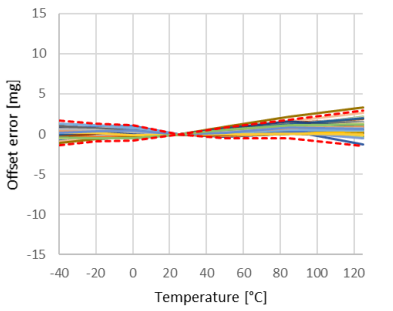
\includegraphics[width=0.45\textwidth]{pictures/tem_x.png}
    }
    \hfill
    \subfloat[Oś OY\label{subfig-4:y}]
    {
      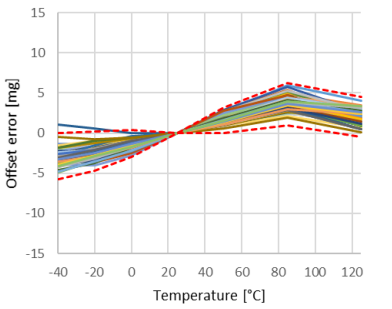
\includegraphics[width=0.45\textwidth]{pictures/tem_y.png}
    }
    \hfill
    \subfloat[Oś OZ\label{subfig-5:z}]
    {
      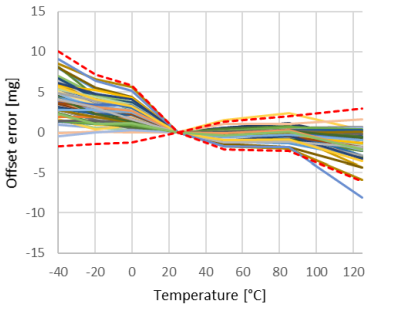
\includegraphics[width=0.45\textwidth]{pictures/tem_z.png}
    }
    \caption{Odchylenia akcelerometru w funkcji temperatury \cite{inclino}}
    \label{fig:inclino_temp}
\end{figure}

Pracuje on na napięciach z zakresu $3.3-3.6$V, możliwe jest więc włączenie go do układu razem z Arduino/Raspberry Pi. Interfejs SPI jest dodatkowym ułatwieniem w komunikacji pomiędzy komponentami.

Przykładowe rozwiązanie:
\begin{itemize}
    \item \href{https://www.mouser.pl/ProductDetail/Murata-Electronics/SCL3300-D01-10?qs=gZXFycFWdAOFydYBLsvu8Q%3D%3D&mgh=1&vip=1&gclid=Cj0KCQiA5NSdBhDfARIsALzs2ECEO9jDFShKG2lA_S2OoNgsOxEbMKKAJx_lWr7MB632r4TBB5kzGLAaAn6aEALw_wcB}{MuRata SCL3300-D01-10}
\end{itemize}